\begin{figure}[H]
	\centering
	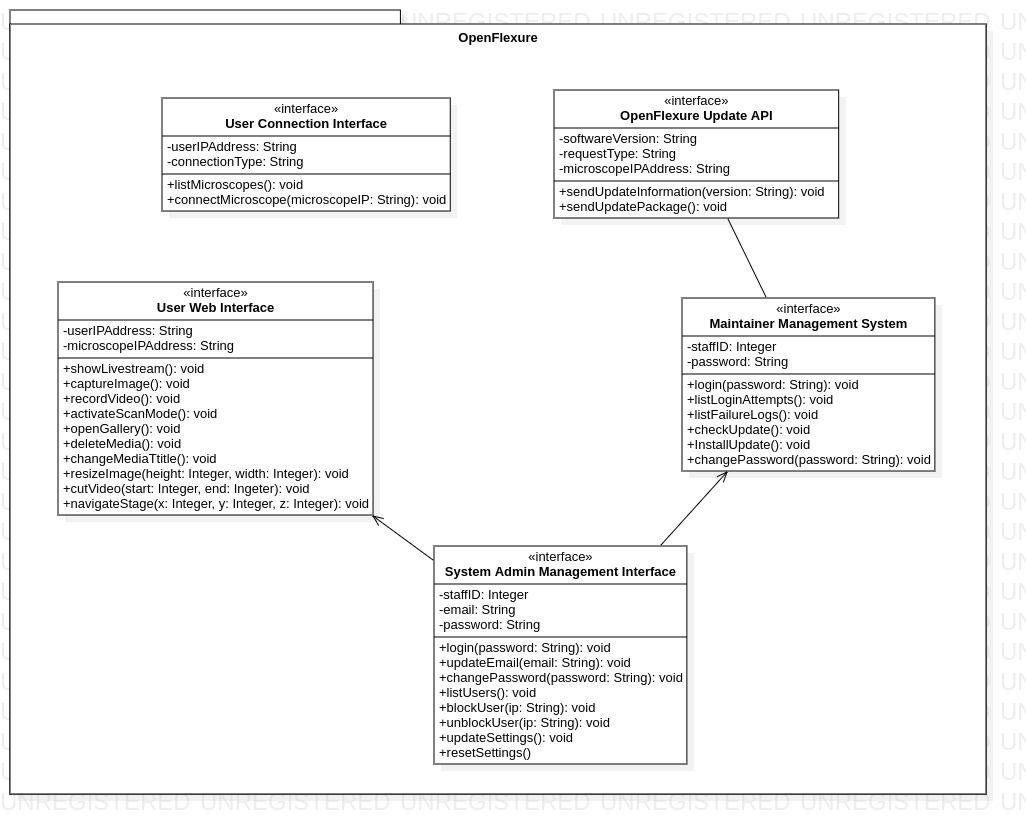
\includegraphics[scale=0.4]{Uml_Images/external_interfaces_class_diagram}
	\caption{External Interfaces Class Diagram}
	\label{fig:external_interfaces_class_diagram}
\end{figure}

\subsubsection{User Connection Interface}
\begin{itemize}
	\item If user chooses connect locally option, this interface displays the path of the Web API. If there is no Web API in the user's computer, then it will display error message.
	\item If user chooses connect remotely, this interface displays the IP addresses and names of the nearby microscopes. There will be option box for each discovered microscope. User will be able to choose the target microscope by clicking on these option boxes.
	\item If there is no microscopes nearby the user, interface will display an error message.
	\item Interface will also displays the  IP addresses the recently connected microscopes.
\end{itemize}

\subsubsection{User Web Interface}
\begin{itemize}
	\item User will be able to view camera feed by clicking the button with the "eye" icon from the side pane. If there is no camera connection, error message will be displayed.
	\item User will be able record the livestream by clicking the "camera" icon from the side pane. Interface will display the recorded video and user will be able to cut the recorded video by entering the start and end time to the textboxes.
	\item User will be able record the livestream by clicking the "camera" icon from the side pane. Interface will display the recorded video and user will be able to cut the recorded video by entering the start and end time to the textboxes.
	\item User will be able capture image from the livestream by clicking the "camera lens" icon from the side pane. Interface will display the captured image and user will be able to resize the captured image by entering the height and width to the textboxes. Furthermore, there will be an option box for scan option. Users will be able to activate scan mode by clicking on this option box.
	\item There will be three textboxes for stage position. User will be able to navigate stage by filling these boxes with coordinates for x, y and z axes.
	\item User will be able to see media save by him/her in grid style gallery format. He/she will be able to view the metadata information by clicking these gallery entries. Furthermore, user will be able to delete media by clicking "delete" button and edit the metadata by clicking "edit" button and filling the corresponding textboxes.
\end{itemize}

\subsubsection{System Admin Management Interface}
\begin{itemize}
	\item Admin will be able to update his/her mail address using this interface. If the email address is invalid (e.g., doesn't contain @ symbol), an error message will be displayed.
	\item Admin will be able to change his/her password. Interface will display "type the new password" text in command-line, then it displays the "confirm new password" text and compare the inputs for these two messages. If the given inputs are not the same, an error message will be displayed.
	\item Admin will be able view current system settings. Interface will receive the setting records from the database and display it in the table format. Then, admin will be able to change the values of the settings by giving the defined commands. If command is invalid, an error message will be displayed. If admin gives "reset settings" command, the system settings in the database will be reset to the default settings.
	\item Admin will be able view connected and blocked users in a detailed list format. By giving the defined commands, he/she will be able to block/unblock users.
\end{itemize}

\subsubsection{Maintainer Management Interface}
\begin{itemize}
	\item Maintainer will be able to change his/her password. Interface will display "type the new password" text in command-line, then it displays the "confirm new password" text and compare the inputs for these two messages. If the given inputs are not the same, an error message will be displayed.
	\item Maintainer will be able to list failed login attempts in a table where each row contains the IP address of the user, attempt time and attempt type (i.e., admin or maintainer attempt).
	\item Maintainer will be able to list failure logs in a table where each row contains the the failure date, failure description, failed system component and severity level of the fail. If the maintainer marks the log as solved, then the log will not be displayed next time.
	\item Maintainer will be able to check whether there is software update or not. OpenFlexure Update API and Maintainer Management Interface will communicate for this task. Maintainer will be able to view the detailed information of the latest software update in command-line interface. Furthermore, he/she will be able to update the system after the checking operation.
\end{itemize}
\subsubsection{OpenFlexure Update API}
\begin{itemize}
	\item When maintainer gives check updates command, Update API shall get the software version and send this information to the OpenFlexure Development Server.
	\item Update API shall get the respond that contains latest update information from the OpenFlexure Development Server.
	\item When maintainer gives update command, Update API shall get the installable update package from the OpenFlexure Development Server.
\end{itemize}